\section{Learning through missing modality}

\label{sec:method}

\begin{frame}{CNN as global descriptor}
	\only<1>
	{
	\begin{figure}
	\centering
	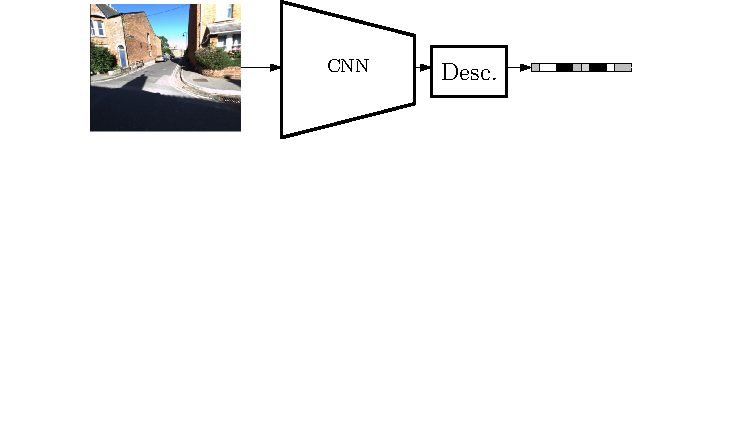
\includegraphics[width=0.7\linewidth]{vect/method/fig2/0n}
	\end{figure}
	\vfill
	\vspace{-1.0cm}
	We use a CNN as trainable global image descriptor\footfullcite{Arandjelovic2017}.
	}
	\only<2>
	{
	\begin{figure}
	\centering
	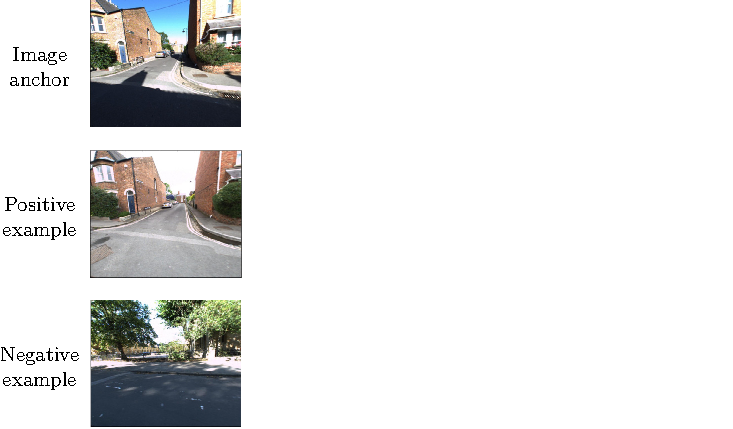
\includegraphics[width=0.7\linewidth]{vect/method/fig2/1}
	\end{figure}
	\vfill
	\textbf{Positive example}: same scene as anchor. \textbf{Negative example}: unrelated to anchor.
	}
	\only<3>
	{
	\begin{figure}
	\centering
	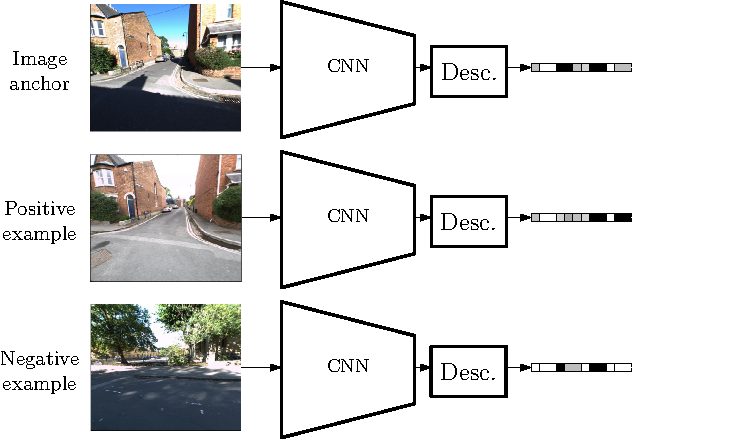
\includegraphics[width=0.7\linewidth]{vect/method/fig2/2n}	
	\end{figure}	
	\vfill
	Descriptors computed with the \textbf{same}	deep descriptor.
	}
	\only<4>
	{
	\begin{figure}
	\centering
	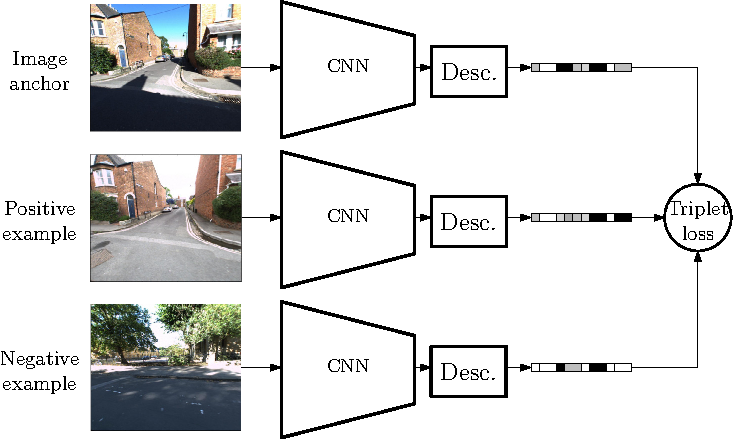
\includegraphics[width=0.7\linewidth]{vect/method/fig2/3n}
	\end{figure}	
	\vfill
	\textbf{Triplet loss} penalizes difference between anchor \& positive example and similarity between anchor \& negative example.
	}
\end{frame}

\begin{frame}{Our method: learning through missing modality}	
	\only<1>
	{
	\begin{minipage}{0.6\linewidth}
		\centering
		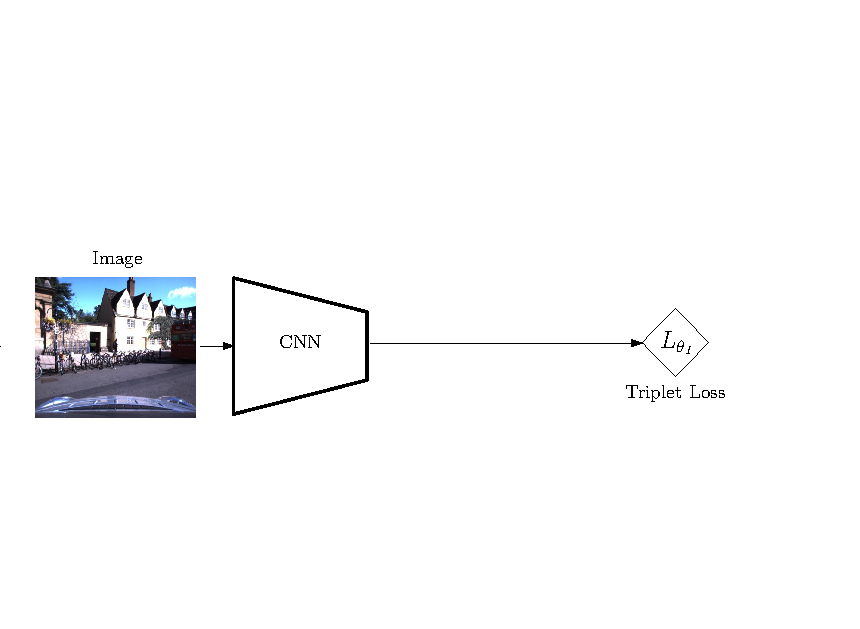
\includegraphics[width=\linewidth]{vect/method/fig3/1}	
	\end{minipage}\hfill
	\begin{minipage}{0.3\linewidth}
		\raggedright
		We use triplet loss to produce strong image descriptor.
	\end{minipage}		
	}
	\only<2>
	{
	\begin{minipage}{0.6\linewidth}
		\centering
		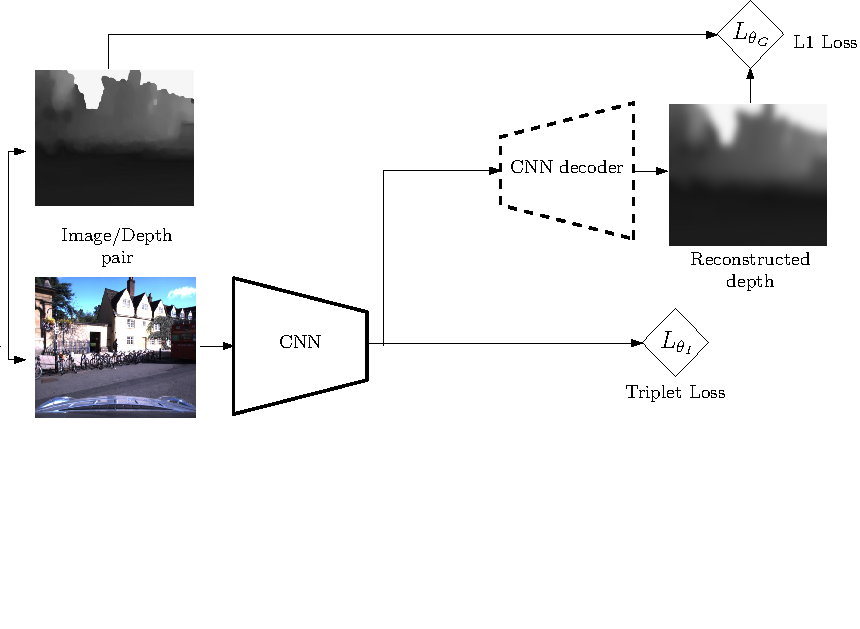
\includegraphics[width=\linewidth]{vect/method/fig3/2}	
	\end{minipage}\hfill
	\begin{minipage}{0.3\linewidth}
		\raggedright
		Latent image representation is given to a CNN decoder to reproduce the scene geometry.\\
		\vspace{0.5cm}
		
		The CNN decoder is simply trained by minimizing $L_{1}$ distance between ground truth and reconstructed depth.
	\end{minipage}		
	
	}
	\only<3>
	{
	\begin{minipage}{0.6\linewidth}
		\centering
		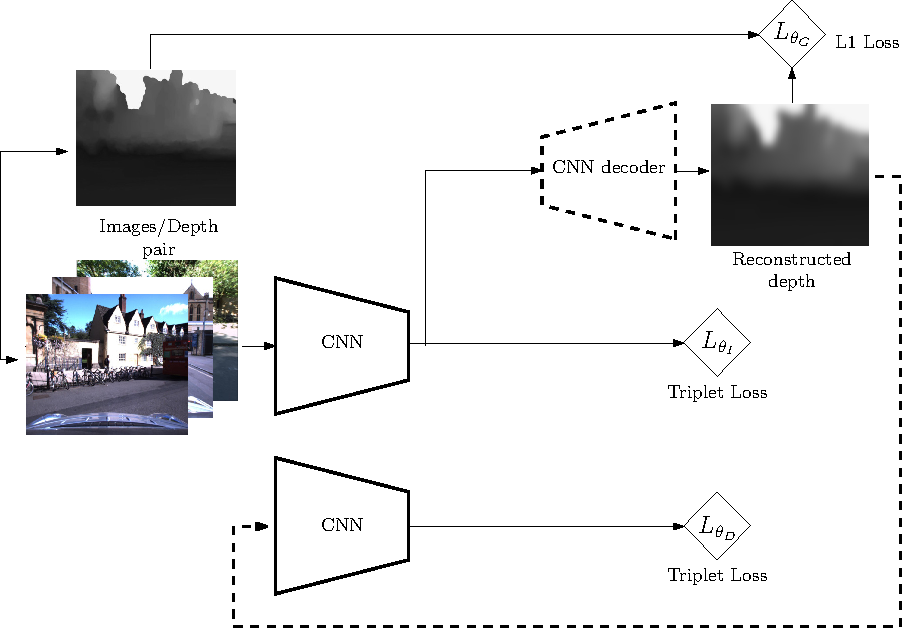
\includegraphics[width=\linewidth]{vect/method/fig3/3}	
	\end{minipage}\hfill
	\begin{minipage}{0.3\linewidth}
		\raggedright
		We use another CNN to produce strong depth map descriptor.
	\end{minipage}			
	
	}
	\only<4>
	{
	\begin{minipage}{0.6\linewidth}
		\centering
		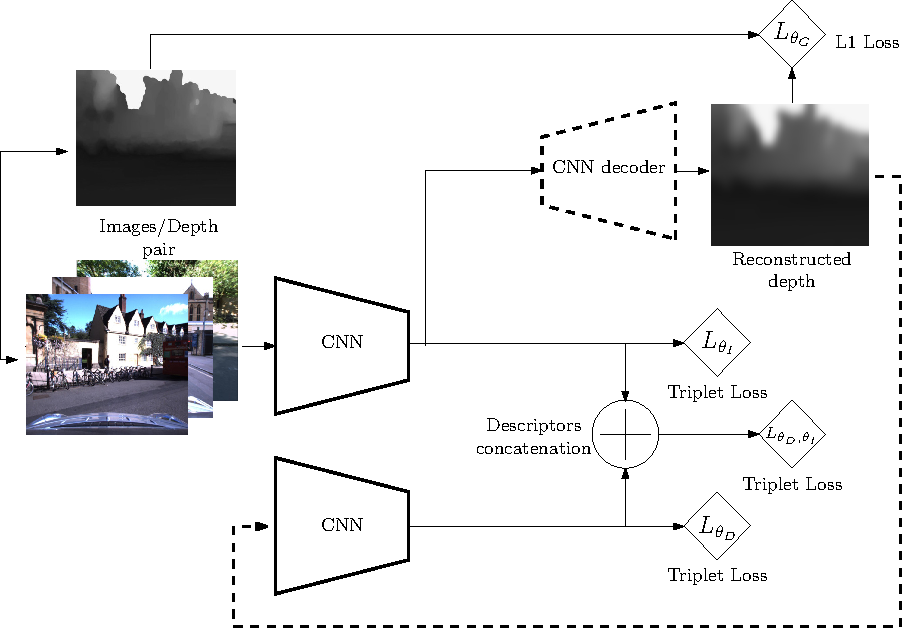
\includegraphics[width=\linewidth]{vect/method/fig3/4}	
	\end{minipage}\hfill
	\begin{minipage}{0.3\linewidth}
		\raggedright
		Final descriptor is obtained by concatenating image and depth map descriptors.
	\end{minipage}			
	
	}
\end{frame}

\begin{frame}{Training policy}
	\only<1>
	{
	\begin{minipage}{0.6\linewidth}
		\centering
		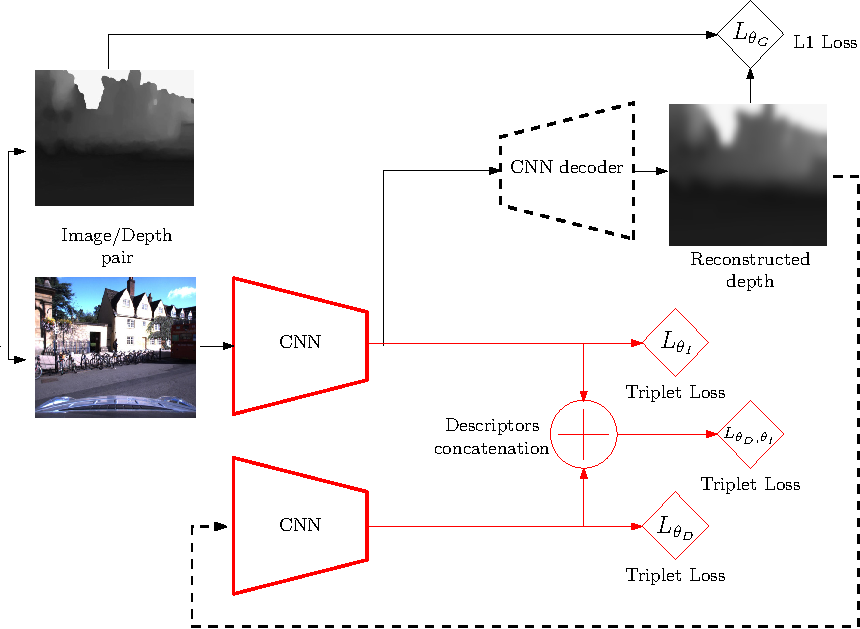
\includegraphics[width=\linewidth]{vect/method/fig3/5}	
	\end{minipage}\hfill
	\begin{minipage}{0.3\linewidth}
		\raggedright
		Data required to train the descriptor part of our system:
		\vspace{0.5cm}
		
		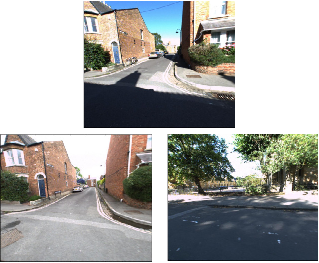
\includegraphics[width=\linewidth]{vect/method/fig3/triplet}	
	\end{minipage}		
	}
	\only<2>
	{
	\begin{minipage}{0.6\linewidth}
		\centering
		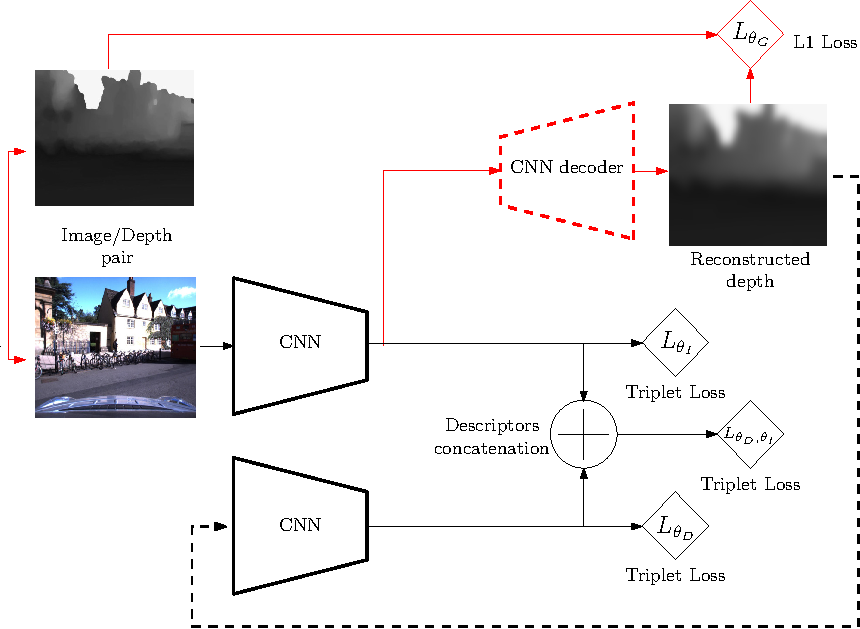
\includegraphics[width=\linewidth]{vect/method/fig3/6}	
	\end{minipage}\hfill
	\begin{minipage}{0.3\linewidth}
		\raggedright
		Data required to train the depth reconstruction part of our system:
		\vspace{0.5cm}
		
		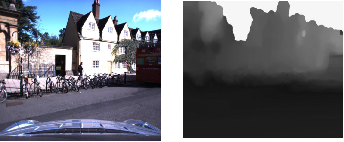
\includegraphics[width=\linewidth]{vect/method/fig3/pair}	
	\end{minipage}			
	}
\end{frame}


\begin{frame}{System deployment}
	\centering
	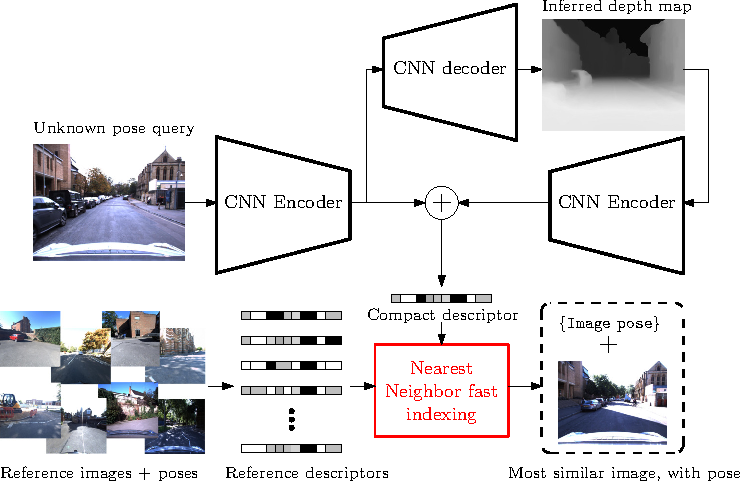
\includegraphics[width=0.7\linewidth]{vect/method/fig4/final}
	\vfill	

	The depth information is only needed during the training step!
\end{frame}